\documentclass[12pt]{article}
\usepackage{amsmath}
\usepackage{amssymb}
\usepackage{lmodern}
\usepackage{xfrac}
\usepackage{enumitem}
\usepackage[dvipsnames]{xcolor}
\usepackage[a4paper,margin=1in]{geometry}
\usepackage[sorting=none,style=nature]{biblatex}
\bibliography{refs}

% commands
\newcommand{\refeq}[1]{Eq.~\eqref{#1}}
\newcommand{\phit}{\frac{\partial \phi}{\partial t}}
\newcommand{\varF}{\frac{\delta F}{\delta \phi}}
\newcommand{\ddphidxx}{\frac{\mathrm{d}^2 \phi}{\mathrm{d} x^2}}
% \newcommand{\deriv}[2]{\frac{\mathrm{d} #1}{\mathrm{d} #2}}
% \newcommand{\dderiv}[2]{\frac{\mathrm{d}^2 #1}{\mathrm{d} #2^2}}
\newcommand{\partiald}[2]{\frac{\partial #1}{\partial #2}}
\newcommand{\diff}{\mathrm{d}}
\providecommand*{\deriv}[3][]{\frac{\diff^{#1}#2}{\diff #3^{#1}}}
\providecommand*{\pderiv}[3][]{\frac{\partial^{#1}#2}{\partial #3^{#1}}}
\newcommand{\dx}{\Delta x}
\newcommand{\dy}{\Delta y}
\newcommand{\dt}{\Delta t}

\title{APC 523 Final Project: Numerically solving the Allen-Cahn equation}
\author{Josh Arrington}
\date{May 07, 2024}

\begin{document}
\maketitle

\section{Introduction and Background}
Phase-field modeling involves a class of modeling used to study physical systems involving interfaces between two distinct phases.
Here, we use "phase" in the materials science sense, referring to a region in space where the system of interest is homogeneous in material properties (composition, mechanical properties, electromagnetic property, structure, etc.).
Material systems in most real-world engineering applications have multiple phases throughout, with the proportion and arrangement of different phases evolving over time.

Consider, for example, a phase-field parameter $\phi\in[-1, 1]$ in a system with two phases, $A$ and $B$, where $\phi=-1$ in phase $A$ and $\phi=1$ in phase $B$.
The historical "sharp interface" approach would view all interfaces between phase $A$ and phase $B$ as points where $phi$ varies discontinuously, in a step-wise manner, between the two phases.
This approach would require different differential equations describing the evolution of some quantitity in the two different phases as well as boundary conditions at the interfaces.
Solving these coupled equations even for two phases is non-trivial, and often non-tractable, because the interfaces and the relevant quantities of interest in the systems are constantly in flux in most systems and processes of interest.
Phase-field modeling seeks to rectify this by allowing the phase-field parameter $\phi$ to vary smoothly and continuously from one phase to another.

One of the classical phase-field models is the Allen-Cahn equation~\cite{allen1972ground,allen1973correction}:
\begin{equation}
    \tau \frac{\partial \phi}{\partial t} = -\frac{\delta F[\phi]}{\delta \phi} \label{eq:allen-cahn}
\end{equation}
where $\phi(\overrightarrow{r}, t)$ is a field parameter of species with spatial and temporal variance, $\tau$ is a control parameter, and $F$ is a free energy functional of $\phi$. The $\delta$ notation refers to a variational derivative (i.e., $\frac{\delta F}{\delta \phi}$ is the variatonal derivative of $F$ with respect to $\phi$).

The Allen-Cahn equation is \textit{non}-conserving for the time evolution of $\phi$, and is used to model other types of phase transitions like solidification in alloys, grain growth, etc \cite{biner2017programming}.
This equation is a gradient flow of the energy functional $F$, and thus requires "energy stability" meaning that $F$ is never increasing as time evolution is being performed ($\frac{\mathrm{d}}{\mathrm{d}t} F[\phi] \leq 0$ for all $t>0$), which is an important property for numerical methods to conserve.

The focus of this project will be on \textbf{the Allen-Cahn Equation, Eq.\eqref{eq:allen-cahn}}, and implementing various numerical methods to solve approximate a solution for an analytical toy problem.

\section{Analytical solution to the Allen-Cahn equation}
Following the literature \cite{provatas2011phase}, I derive an analytical solution to the Allen-Cahn equation.
In this work, I consider a pure system with one component whose order is represented by $\phi$ with two phases at $\phi=\pm 1$.
To accomodate diffuse interfaces, the free energy functional considered here is of the form
\begin{equation}
    F[\phi] = \int_V \left(f(\phi) + \frac{w^2}{2}(\nabla \phi)^2\right) \mathrm{d}V \label{eq:functional}
\end{equation}
which consists of a bulk free energy functional, $f(\phi)$, and the lowest-order term to account for local variations \cite{cahn1958free} in the phase field.
The parameter $w$ is representative of the mobility of the species.
To promote a two-phase solution, a so-called "double well" bulk free energy functional is considered:
\begin{equation}
    f(\phi) = -\frac{1}{2}\phi^2 + \frac{1}{4}\phi^4 + H (\phi-\frac{1}{3}\phi^3)
\end{equation}
with minima at $\phi = \pm 1$. 
$H$ controls the asymmetry of the two minima in the region $\phi \in [-1, 1]$.
This role of $H$ is seen in Figure~\ref{fig:energy_well}, where a positive value skews the minima at $\phi=-1$ lower than the minima at $\phi = 0$.

\begin{figure}
    \centering
    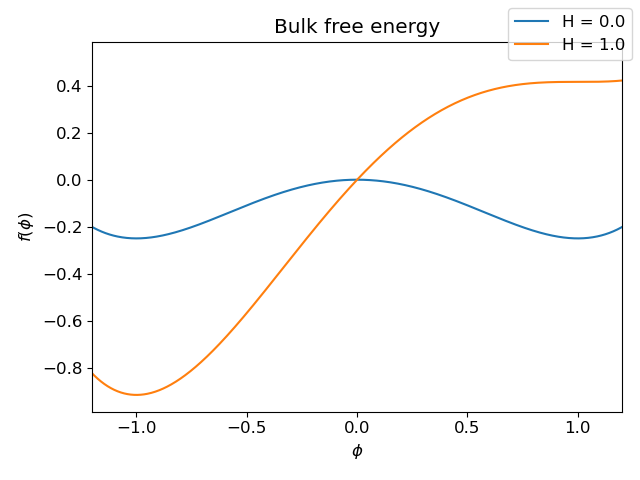
\includegraphics[width=0.5\textwidth]{../figures/energy_well.png}
    \caption{Bulk free energy functional with $H = 0$ (blue) and $H = 1$ (orange)}
    \label{fig:energy_well}
\end{figure}

With this chose form of our free energy functional, then upon taking the variational derivative of \refeq{eq:functional} the Allen-Cahn equation becomes
\begin{equation}
    \tau \phit = w^2 \nabla^2 \phi + \phi - \phi^3 - H(1-\phi^2)
    \label{eq:AC_general}
\end{equation}

\subsection{1D Allen-Cahn equation}\label{sec:1D_ac}
Let us consider the 1D case first, where $x$ denotes our spatial variable extending from $-\infty$ to $\infty$.
At steady state and when $H = 0$, $\phit \rightarrow 0$ and \refeq{eq:AC_general} becomes
\begin{equation}
    w^2 \ddphidxx +\phi - \phi^3 = 0 \label{eq:1d_equil}
\end{equation}
Then an equilibrium solution to \refeq{eq:AC_general} in 1D is clearly:
\begin{equation}
    \phi_{eq}(x) = \tanh{\left(\frac{x}{\sqrt{2}w}\right)}
\end{equation}
We can verify this:
\begin{align}
    \frac{\mathrm{d}^2 \phi_{eq}}{\mathrm{d}x^2} = -\frac{1}{w^2}\left(\tanh{\left(\frac{x}{\sqrt{2}w}\right) - \tanh^3{\left(\frac{x}{\sqrt{2}w}\right)}}\right) \nonumber \\
    \implies -\frac{w^2}{w^2}\left(\tanh{\left(\frac{x}{\sqrt{2}w}\right) - \tanh^3{\left(\frac{x}{\sqrt{2}w}\right)}}\right) + \phi_{eq} - \phi_{eq}^3 = 0 \nonumber
\end{align}


We can interpret this 1D solution physically as a smooth transition from $\phi = -1$ to $\phi = 1$, and we can define an interface as the point where $\phi = 0$ (for the purpose of tracking the interface's motion).
Thus, with an initial state of the form of \refeq{eq:1d_equil}, then $\phit = 0$ and the system would be stagnant (the interface ).
However, if $H \neq 0$, then we would have a driving force for the motion of the interface between the two phases and $\phit \neq 0$.

Let us consider $H>0$ but not too large. 
It has been shown in the literature that such a scenario results in a solution that the interface propagating at constant speed $v$.
Following \cite{provatas2011phase}, we can recover this result through the method of characteristics, similar to the advection equation.
We approximate $\phi(x,t) \approx \phi_{eq}(x-vt) = \phi(u)$ and define $u\equiv x-vt$.
Then, the 1D Allen-Cahn equation becomes
\begin{equation}
    \tau \deriv{\phi_{eq}}{u} \pderiv{u}{t} = -v \tau \deriv{\phi_{eq}}{u} = w^2 \deriv[2]{\phi_{eq}}{u} + \phi_{eq} - \phi_{eq}^3 -H\left(1 - \phi_{eq}^2\right) \label{eq:1d_nonzero_H}
\end{equation}
However, by construction, the first three terms on the right-hand side of \refeq{eq:1d_nonzero_H} combine to 0 (since $\phi_{eq}$ is a solution to \refeq{eq:1d_equil}).
Thus, we can write
\begin{equation}
    -v\tau \deriv{\phi_{eq}}{u} = -H\left(1-\phi_{eq}^2\right)
    \label{eq:dphidu}
\end{equation}

To derive what the constant velocity of the interface $v$ is, we use the trick of integrating over both sides of \refeq{eq:dphidu} with $\deriv{\phi_{eq}}{u}$ as our "kernel":
\begin{align}
    \int_{-\infty}^{\infty} \left(\deriv{\phi_{eq}}{u} \left(-v \tau \deriv{\phi_{eq}}{u}\right)\right)\diff u &= \int_{-\infty}^{\infty} \left(-H (1-\phi_{eq}^2)\right)\diff u \nonumber \\
    -v \tau \int_{-\infty}^{\infty}\left(\deriv{\phi_{eq}}{u}\right)^2 \diff u &= -H \int_{-\infty}^{\infty} \frac{\diff}{\diff u} \left(\phi_{eq} - \frac{1}{3}\phi_{eq}^3\right)\diff u \nonumber \\
    -v \tau \int_{-\infty}^{\infty}\left(\deriv{\phi_{eq}}{u}\right)^2 \diff u &= -H \left.\left(\phi_{eq} - \frac{1}{3}\phi_{eq}^3\right)\right|_{-\infty}^{\infty} \nonumber \\
    \implies v &= \frac{4H}{3\tau}\left(\int_{-\infty}^{\infty}\left(\deriv{\phi_{eq}}{u}\right)^2 \diff u\right)^{-1} \label{eq:1d_vel}
\end{align}
We see that the velocity is indeed constant and proportional to the controlling parameters $H, \tau, w$.

\subsection{2D Allen-Cahn equation}\label{sec:2D_ac}
Now, consider a perfectly circular domain in 2D with $\phi=1$ inside the domain, and $\phi = -1$ outside the domain.
Following the above analysis and again utilizing the method of characteristics, we assume that $\phi(r,t) \approx \phi_{eq}(r-R(t))$ where $r$ is the initial domain radius and $R(t)$ is the radius of the domain at time $t$.
Taking the laplacian in polar coordinates, we are led to the 2D Allen-Cahn equation for this scenario as
\begin{align}
    -\tau \deriv{\phi_{eq}}{u}\deriv{R}{t} &= w^2 \deriv[2]{\phi_{eq}}{u} + \phi_{eq} -\phi_{eq}^3 - H \left(1-\phi_{eq}^2\right) + \frac{1}{r}\deriv{\phi_{eq}}{u} \nonumber \\
    \implies -\tau \deriv{\phi_{eq}}{u}\deriv{R}{t} &=  - H \left(1-\phi_{eq}^2\right) + \frac{1}{r}\deriv{\phi_{eq}}{u} \label{eq:2d_ac}
\end{align}
where again the first three terms on the right-hand side sum to zero by construction of $\phi_{eq}$.

Again, integrating over both sides with the kernel $\deriv[]{\phi_{eq}}{u}$:
\begin{align}
    -\int_{-\infty}^{\infty}\left(\tau \deriv[]{R}{t} \left(\deriv[]{\phi_{eq}}{u}\right)^2\right)\diff u &= \frac{1}{r} \int_{-\infty}^{\infty}\left(\deriv{\phi_{eq}}{u}\right)^2 \diff u - H \int_{-\infty}^{\infty} \frac{\diff}{\diff u} \left(\phi_{eq} - \frac{1}{3}\phi_{eq}^3\right)\diff u \nonumber \\
    -\tau \alpha \deriv[]{R(t)}{t} &= \frac{\alpha}{r} - \frac{4H}{3} \nonumber \\
    \implies \deriv[]{R(t)}{t} &= -\frac{1}{\tau R(t)} + \frac{4H}{3\tau\alpha} \label{eq:R_t}
\end{align}
where in the second line we defined $\alpha \equiv \int_{-\infty}^{\infty}\left(\deriv{\phi_{eq}}{u}\right)^2 \diff u$.

\refeq{eq:R_t} holds for all $H\neq 0$ that are not too large in magnitude.
For further analysis, we consider the case when $H=0$.
Then, \refeq{eq:R_t} becomes
\begin{align}
    \deriv[]{R(t)}{t} &= -\frac{1}{\tau R(t)} \nonumber \\
    R(t)^2 - R(0)^2 &= -\frac{2t}{\tau} \nonumber \\
    \implies A(t) &= A(0) - \frac{2t}{\tau} \label{eq:2d_area}
\end{align}
where in the second line we solved the ODE by separation of variables and in the third line we multiplied both sides by $\pi$ to get the area of the circular domain.
Thus, \refeq{eq:2d_area} predicts that even for a symmetric bulk free energy ($H=0$), the circular domain would shrink for $\tau>0$.
The physical interpretation for this is that surface tension results in an energetic cost for a curved interface in 2D.

\section{Numerical Algorithms}
For both the 1D and 2D cases, I implement the following numerical algorithms:
\begin{itemize}
    \item Finite difference solver with explicit Forward Euler (FE) time-stepping
    \item Finite difference solver with fourth-order Runge-Kutta (RK4) time-stepping
    \item Spectral methods with semi-implicit methods
\end{itemize}
This was done in Python 3.12.2 with the standard scientific libraries of Numpy, Matplotlib, and Scipy.
\subsection{1D numerical algorithms}
In 1D, space is discretized as $x_i \in [0, L], \; i=0,\dots,N$.
The spatial resolution is then $\dx = L / N$.
For our 1D case, the finite-difference FE algorithm is quite straight forward.
We approximate the second derivative $\deriv[2]{\phi}{x}$ using the fourth-order, five-point central finite difference stencil:
\begin{equation}
    \deriv[2]{\phi(x_i^n)}{x} \approx \frac{-\phi_{i+2}^n+16\phi_{i+1}^n-30\phi_{i}^n+16\phi_{i-1}^n - \phi_{i-2}^n}{12(\dx)^2}
    \label{eq:1d_lap}
\end{equation}
For $\phi_i$ near the boundary, the boundary values are extended to imitate a semi-infinite domain.
Then the explicit FE solver for the 1D \refeq{eq:AC_general} is simply
\begin{align}
    \tau \frac{\phi_i^{n+1} - \phi_i^n}{\dt} &= w^2 \frac{-\phi_{i+2}^n+16\phi_{i+1}^n-30\phi_{i}^n+16\phi_{i-1}^n - \phi_{i-2}^n}{12(\dx)^2} - f'(\phi_i^n) \label{eq:1d_FE} \\
    -f'(\phi_i^n) &= \phi_i^n - (\phi_i^n)^3 - H(1-(\phi_i^n)^2) \label{eq:bulk_deriv}
\end{align}

However, we know that FE is both restrictive on the timestep, as well as first-order accurate.
From Lecture 13, we know that RK4 has a wider stability region (and can thus make larger timesteps) and is also fourth-order accurate.
The RK4 algorithm for the 1D Allen-Cahn equation then becomes:
\begin{align}
    g(\phi_i^n) &\equiv \frac{1}{\tau}\left(w^2 \frac{-\phi_{i+2}^n+16\phi_{i+1}^n-30\phi_{i}^n+16\phi_{i-1}^n - \phi_{i-2}^n}{12(\dx)^2} + f'(\phi_i^n)\right) \nonumber \\
    \phi_1 &= \phi^n, \; k_1 = g(\phi_1) \nonumber \\
    \phi_2 &= \phi^n + \frac{\dt}{2}k_1, \; k_2 = g(\phi_2) \nonumber \\
    \phi_3 &= \phi^n + \frac{\dt}{2}k_2, \; k_3 = g(\phi_3) \nonumber \\
    \phi_4 &= \phi^n + k_3 \dt, \; k_4 = g(\phi_4) \nonumber \\
    \phi^{n+1} &= \phi^n + \frac{\dt}{6}\left(k_1 + 2k_2 + 2k_3 + k_4\right) \label{eq:1d_rk4}
\end{align}
Note that the numbered subscripts in the stages refer to the global \textit{stage} and not the discrete value of $\phi$ at that index.

Finally, the semi-implicit spectral method (following \cite{biner2017programming}) treats the linear and second-order terms implicitly and the nonlinear $f'(\phi)$ terms explicitly.
We denote the Fourier transform of $\phi$ as $\left\{\phi\right\}_k$ and recognize that 
\begin{equation*}
    \left\{\pderiv[n]{\phi}{x}\right\}_k = \left(\left(\sqrt{-1}\right)k\right)^n \left\{\phi\right\}_k
\end{equation*}
Then, the semi-implicit spectral form of \refeq{eq:AC_general}
\begin{align}
    \tau \frac{\left\{\phi_i\right\}_k^{n+1} - \left\{\phi_i\right\}_k^{n}}{\dt} & = -\left\{f'(\phi_i)\right\}_k^n - k^2 w^2 \left\{\phi_i\right\}_k^{n+1} \nonumber \\
    \implies \left\{\phi_i\right\}_k^{n+1} & = \frac{\left\{\phi_i\right\}_k^n - \frac{\dt}{\tau}\left\{f'(\phi_i)\right\}_k^n}{1 + \frac{\dt}{\tau} k^2 w^2 } \label{eq:1d_spectral}
\end{align}
To enforce periodic boundary conditions in the 1D system, the domain of simulation is mirrored across the right boundary.
It is important to note that due to the nonlinearity of $f'(\phi)$, it is evaluated in real space at each time step.
This means that at each timestep, the spectral method requires:
\begin{enumerate}
    \item Fourier transform $\phi_i^n$ and $f'(\phi_i^n)$. 
    \item Evaluate \refeq{eq:1d_spectral}
    \item Inverse Fourier transform $\left\{\phi_i\right\}_k^{n+1}$
\end{enumerate}
This can become expensive as systems reach large $N$.

\subsection{2D numerical algorithms}
In 2D, space is discretized as $(x_i, y_j) \in [0, L] \times [0, L],\; i, j = 0, \dots, N$.
This is a square domain and the spatial resolution is $\dx = \dy = L/N \equiv h$.
The Laplacian is approximated using the second-order 5-point central difference approximation:
\begin{equation}
    \nabla^2 \phi_{i,j}^n \approx \frac{\phi_{i+1, j}^n + \phi_{i-1, j}^n + \phi_{i, j+1}^n + \phi_{i, j-1}^n - 4\phi_{i,j}^n}{h^2}
\end{equation}
Again, for $\phi_{i,j}$ near the boundary, the boundary values are extended to imitate a semi-infinite domain.
Then the explicit FE solver for the 2D \refeq{eq:AC_general} is simply
\begin{align}
    \tau \frac{\phi_{i,j}^{n+1} - \phi_{i,j}^n}{\dt} &= w^2 \frac{\phi_{i+1, j}^n + \phi_{i-1, j}^n + \phi_{i, j+1}^n + \phi_{i, j-1}^n - 4\phi_{i,j}^n}{h^2} - f'(\phi_{i,j}^n)  \label{eq:2d_fe} \\
    -f'(\phi_{i,j}^n) &= \phi_{i,j}^n - (\phi_{i,j}^n)^3 - H(1 - (\phi_{i,j}^n)^2)
\end{align}
Similarly, the RK4 algorithm for the 2D Allen-Cahn equation then becomes:
\begin{align}
    g(\phi_{i,j}^n) &\equiv \frac{1}{\tau}\left(w^2 \frac{\phi_{i+1, j}^n + \phi_{i-1, j}^n + \phi_{i, j+1}^n + \phi_{i, j-1}^n - 4\phi_{i,j}^n}{h^2} - f'(\phi_{i,j}^n)\right) \nonumber \\
    \phi_1 &= \phi^n, \; k_1 = g(\phi_1) \nonumber \\
    \phi_2 &= \phi^n + \frac{\dt}{2}k_1, \; k_2 = g(\phi_2) \nonumber \\
    \phi_3 &= \phi^n + \frac{\dt}{2}k_2, \; k_3 = g(\phi_3) \nonumber \\
    \phi_4 &= \phi^n + k_3 \dt, \; k_4 = g(\phi_4) \nonumber \\
    \phi^{n+1} &= \phi^n + \frac{\dt}{6}\left(k_1 + 2k_2 + 2k_3 + k_4\right) \label{eq:2d_rk4}
\end{align}
Again, note that the numbered subscripts in each stage of the RK4 algorithm refer to the global stage and not the discrete value of $\phi$ at that index.

Finally, the semi-implicit spectral method in 2D for the Allen-Cahn equation is trivially similar to \refeq{eq:1d_spectral}:
\begin{equation}
    \left\{\phi_{i,j}\right\}_k^{n+1}  = \frac{\left\{\phi_{i,j}\right\}_k^n - \frac{\dt}{\tau}\left\{f'(\phi_{i,j})\right\}_k^n}{1 + \frac{\dt}{\tau} k^2 w^2 } \label{eq:2d_spectral}
\end{equation}
For the 2D simulations, the domain involves a circular region of $\phi = 1$ in the center and $\phi=-1$ outside of this circle (with a smooth, diffuse transition between them) and so the artificial periodicity needed for the spectral method is naturally accounted for since the domain is symmetric in the radial direction.
However, since we do not mirror the domain as in the 1D case, then in 2D we have half of the wavevectors in Fourier space for the same spatial resolution compared to the 1D case (although the Nyquist frequency is the same).
The magnitude of the wavevectors in 2D are given as
\begin{equation}
    k^2 = k_x^2 + k_y^2
\end{equation}

\section{Results and Discussion}
For both the 1D and 2D case, the parameters $\tau, w, H$ were all set to unity unless otherwise specified.
The spatial resolution is $h = L / N$ and the temporal resolution is set to $\dt \approx h/100$. 
Although the RK4 and spectral methods can handle temporal resolution greater than this, it was chosen for stability of the FE algorithm and for consistent comparison of the accuracy of all three methods.

\subsection{1D results}
In 1D, $N = [32, 64, 128, 256, 512]$.
For all 1D cases, we compare numerical profiles of $\phi$ versus the known analytical solution discussed in Sec.~\ref{sec:1D_ac}:
\begin{equation}
    \phi(x,t) = \phi_{eq}(x-vt) = \tanh \left(\frac{x - vt}{\sqrt{2} w}\right)
\end{equation}
where $v$ is analytically calculated according to \refeq{eq:1d_vel}.
Evolutions of the profile using FE, RK4, and FFT/spectral methods are shown in Figs.~\ref{fig:FE_prof},~\ref{fig:RK4_prof}, and~\ref{fig:FFT_prof} respectively for $N=32$.

The accuracy of a method is calculated by comparing the profile from the numerical evolution to the profile analytically calculated from the theory using the $L^2$ norm:
\begin{equation}
    e_{L^2} (t) = \int_{0}^{L} |\phi_{\text{approx}}(x,t) - \phi_{\text{exact}}(x,t)| \diff x 
    \label{eq:L2_norm}
\end{equation}
\begin{figure}
    \centering
    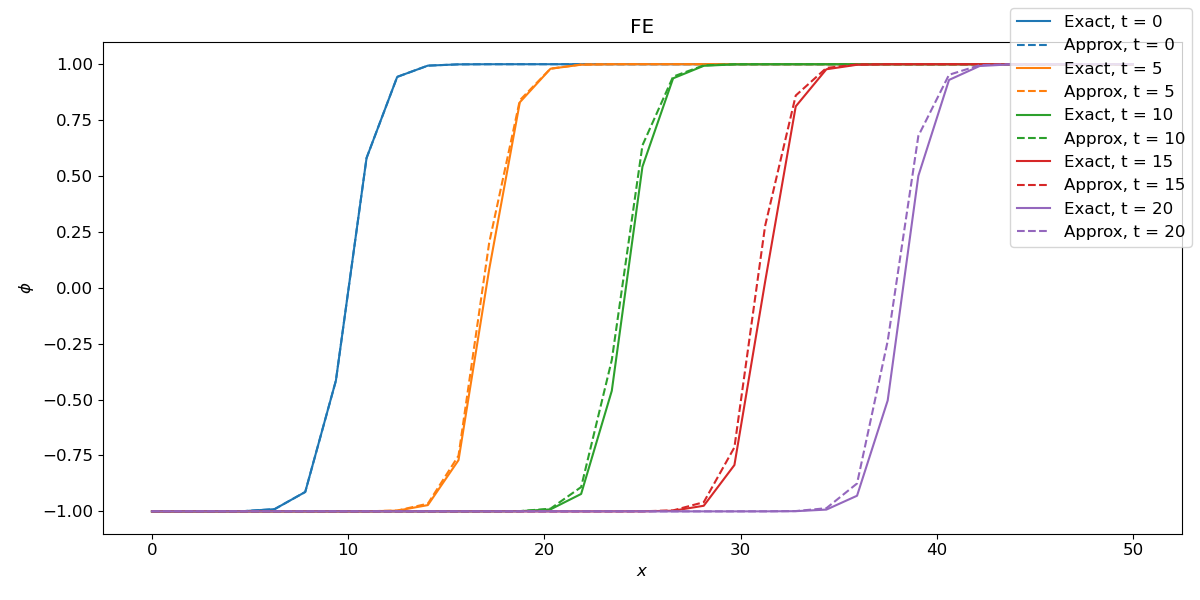
\includegraphics[width=0.7\textwidth]{../figures/FEprof_evo.png}
    \caption{Evolution of profile with FE algorithm}
    \label{fig:FE_prof}
\end{figure}
\begin{figure}
    \centering
    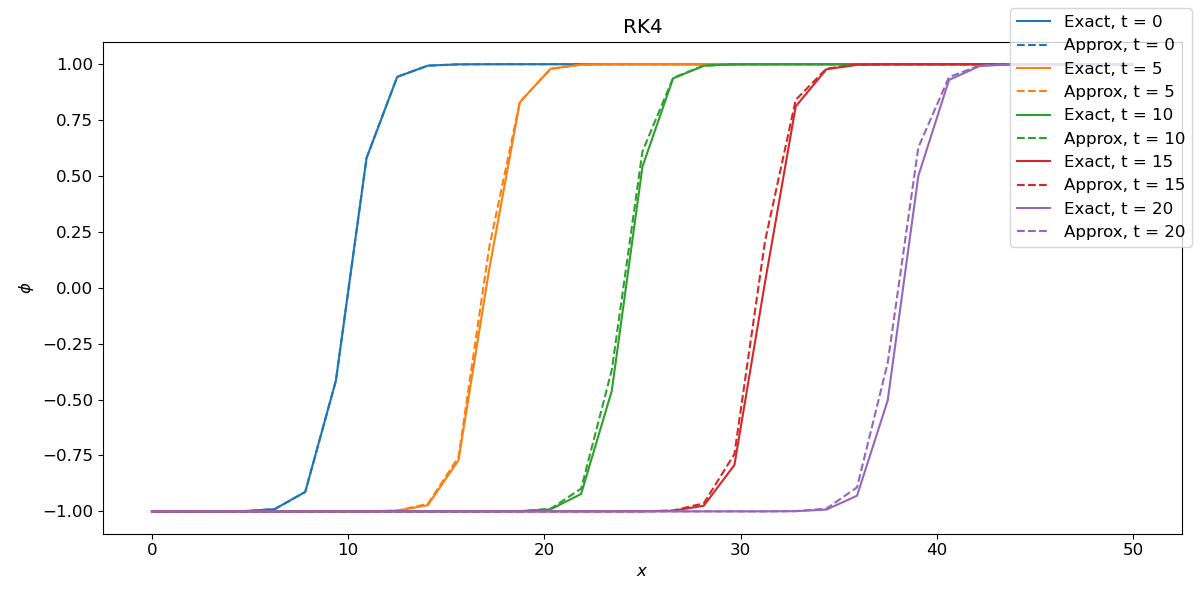
\includegraphics[width=0.7\textwidth]{../figures/RK4prof_evo.png}
    \caption{Evolution of profile with RK4 algorithm}
    \label{fig:RK4_prof}
\end{figure}
\begin{figure}
    \centering
    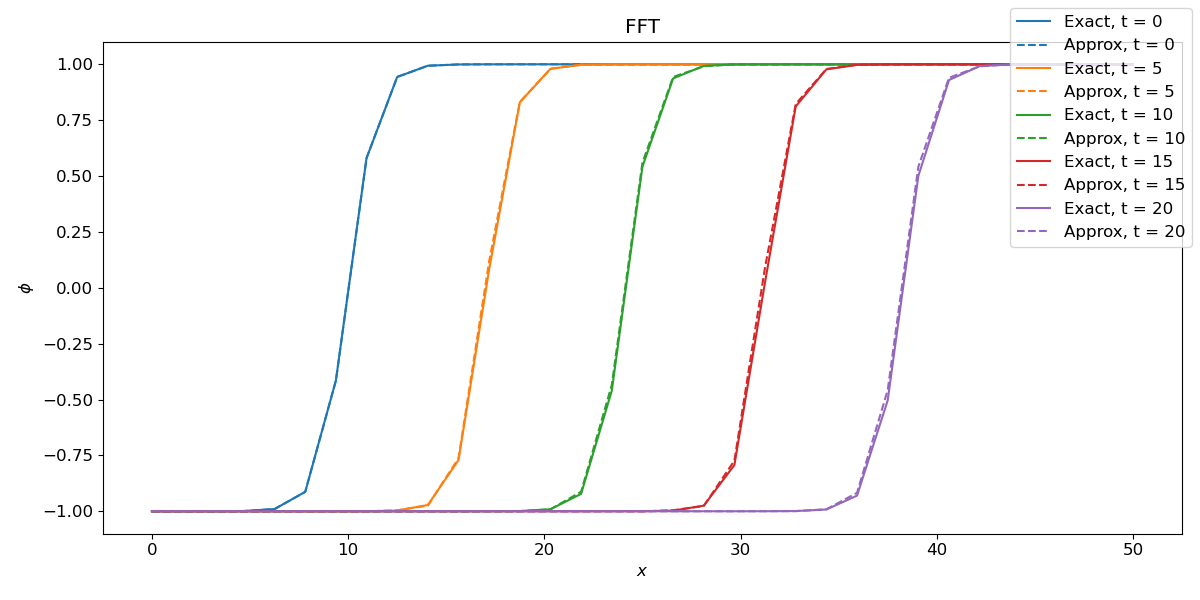
\includegraphics[width=0.7\textwidth]{../figures/FFTprof_evo.png}
    \caption{Evolution of profile with FFT algorithm}
    \label{fig:FFT_prof}
\end{figure}
\begin{figure}
    \centering
    \begin{minipage}{0.3\textwidth}
        \centering
        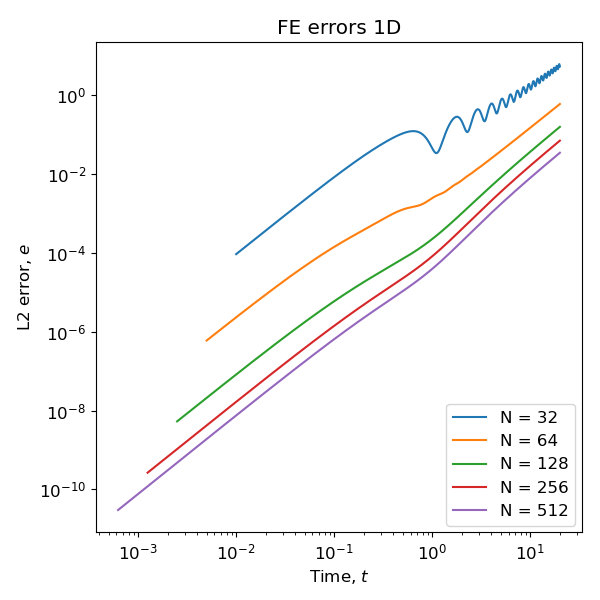
\includegraphics[width=0.99\textwidth]{../figures/FE_errors_1D.png}
        \caption{1D FE error vs time}
        \label{fig:1d_fe_err}
    \end{minipage}\hfill
    \begin{minipage}{0.3\textwidth}
        \centering
        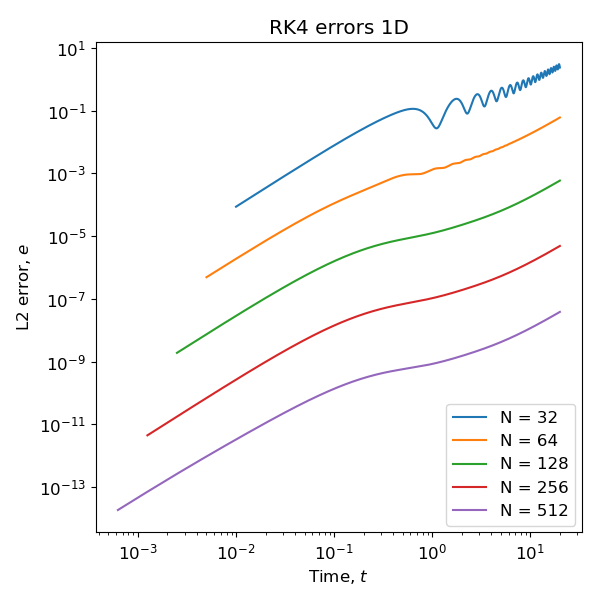
\includegraphics[width=0.99\textwidth]{../figures/RK4_errors_1D.png}
        \caption{1D RK4 error vs time}
        \label{fig:1d_rk4_err}
    \end{minipage}\hfill
    \begin{minipage}{0.3\textwidth}
        \centering
        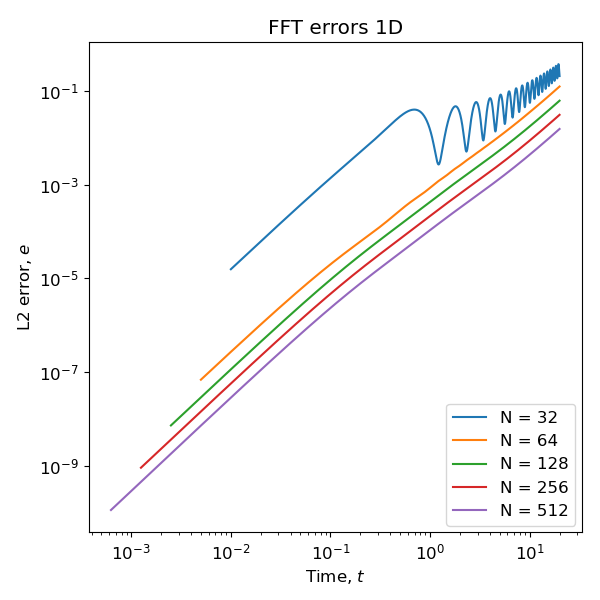
\includegraphics[width=0.99\textwidth]{../figures/FFT_errors_1D.png}
        \caption{1D FFT error vs time}
        \label{fig:1d_fft_err}
    \end{minipage}\hfill
\end{figure}
\begin{figure}
    \centering
    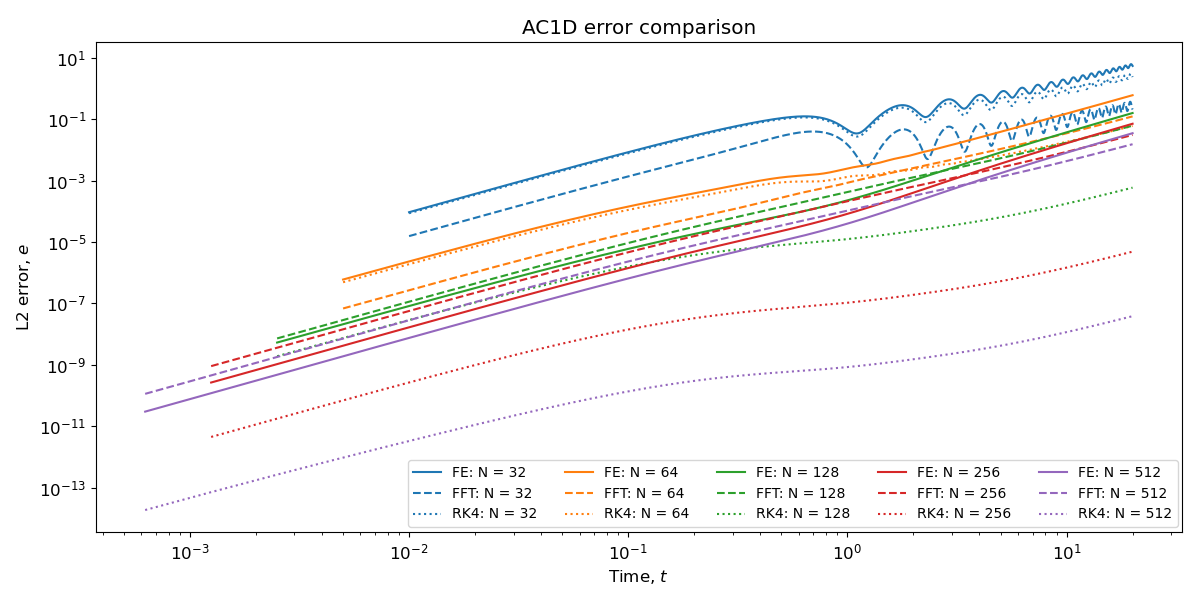
\includegraphics[width=0.9\textwidth]{../figures/AC1D_error_comparison.png}
    \caption{1D error vs time for the three numerical algorithms}
    \label{fig:1d_error_comparison}
\end{figure}
In Figs.~\ref{fig:1d_fe_err} through~\ref{fig:1d_fft_err} we see the individual error versus time plots for the three algorithms with varying number of spatial grid points.
For direct comparison, all three algorithms' error versus time are plotted on Fig.~\ref{fig:1d_error_comparison}.
For low $N$, the spectral method has superior accuracy due to the exponential convergence of the spectral methods.
However, for large $N$, the fourth-order nature of RK4 allows it to become the most accurate.

As discussed above, RK4 is a multistage method and the spectral method requires both a forward and an inverse Fourier transform (which is $\mathcal{O}(N \log N)$).
Thus, we compare the execution time for each method in Fig.~\ref{fig:1d_exec_time}.
Clearly, RK4 is the most expensive computationally since it has 4 stages per timestep.
However, it is the most accurate method and thus would be preferred for long time simulations.

\begin{figure}
    \centering
    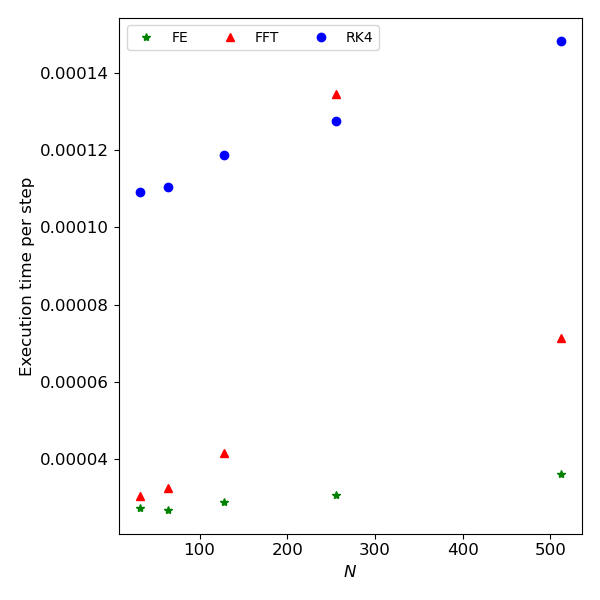
\includegraphics[width=0.5\textwidth]{../figures/AC1D_exec_time.png}
    \caption{Execution times of the various 1D numerical methods}
    \label{fig:1d_exec_time}
\end{figure}

\subsection{2D results}
In 2D, $N = [64, 128, 256]$ for computational speed for demonstration.
For the 2D cases, we set $H=0$ for direct comparison against \refeq{eq:2d_area}.
The initial state is given as 
\begin{equation}
    \phi(r,0) = -\tanh \left(\frac{r-R_0}{\sqrt{2} w}\right) \label{eq:2d_init}
\end{equation}
(\textit{Note: videos of $H=1.0$ are shown in the slides/Github}).

To analyze the accuracy of the 2D algorithms, the radius of the circle where $\phi = 0$ is found and then used to compute an approximate area, $A_{approx} = \pi (r_{\phi=0})^2$.
This is directly compared to $A_{exact}$ as calculated via \refeq{eq:2d_area}:
\begin{equation}
    e_{\text{max}}(t) = |A_{approx}(t) - A_{exact}(t)| \label{eq:2d_error}
\end{equation}
\begin{figure}
    \centering
    \begin{minipage}{0.3\textwidth}
        \centering
        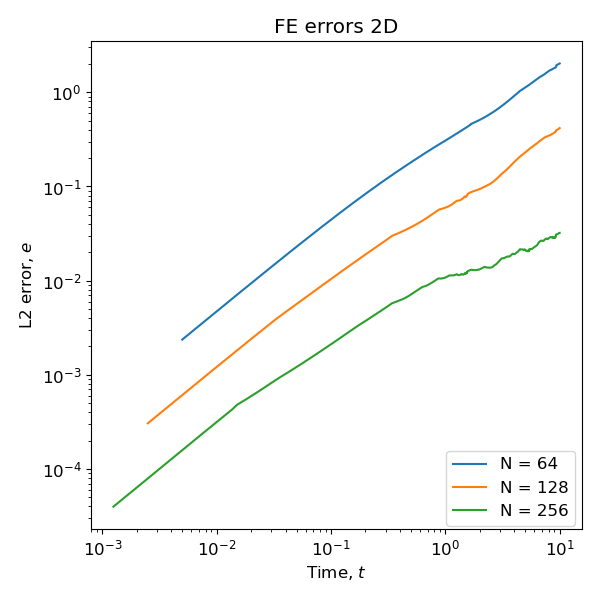
\includegraphics[width=0.99\textwidth]{../figures/FE_errors_2D.png}
        \caption{2D FE error vs time}
        \label{fig:2d_fe_err}
    \end{minipage}\hfill
    \begin{minipage}{0.3\textwidth}
        \centering
        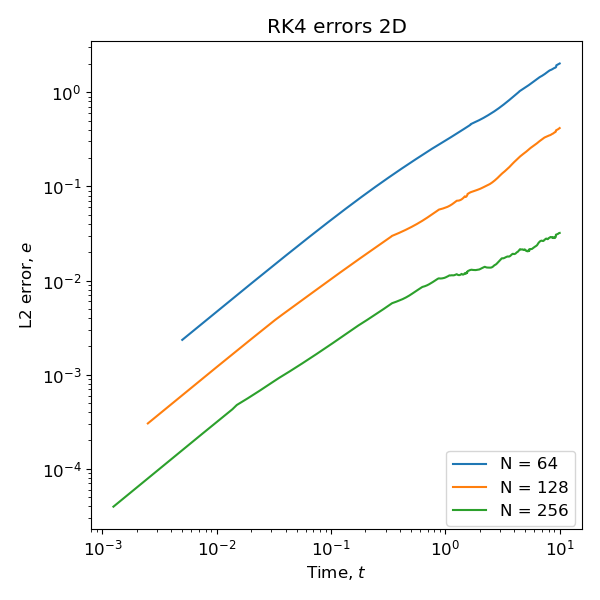
\includegraphics[width=0.99\textwidth]{../figures/RK4_errors_2D.png}
        \caption{2D RK4 error vs time}
        \label{fig:2d_rk4_err}
    \end{minipage}\hfill
    \begin{minipage}{0.3\textwidth}
        \centering
        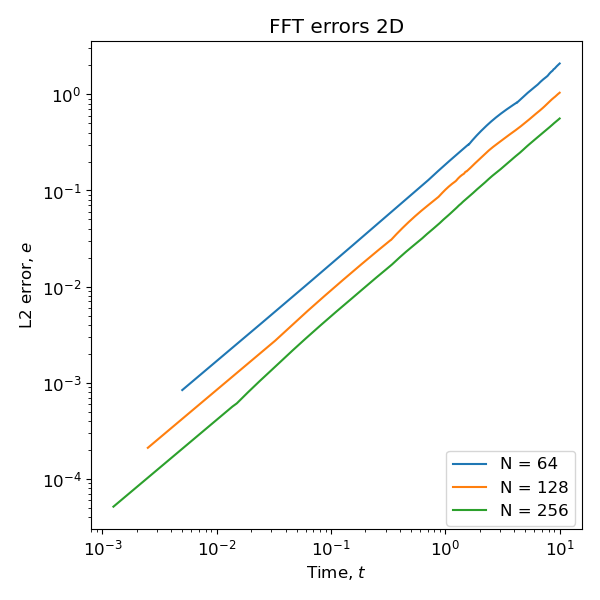
\includegraphics[width=0.99\textwidth]{../figures/FFT_errors_2D.png}
        \caption{2D FFT error vs time}
        \label{fig:2d_fft_err}
    \end{minipage}\hfill
\end{figure}
\begin{figure}
    \centering
    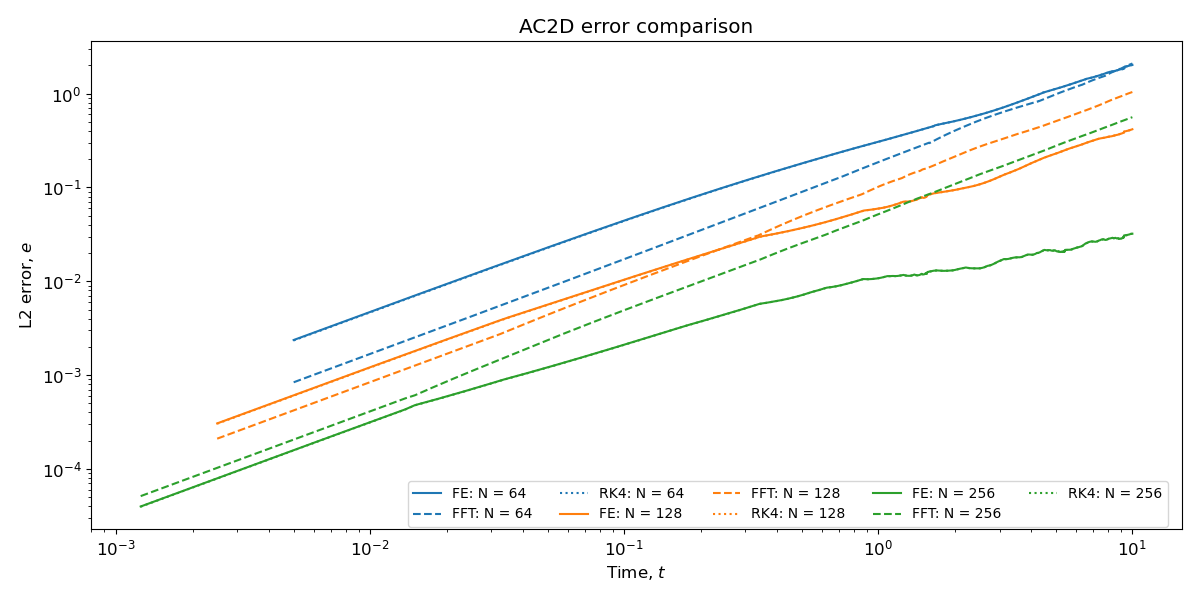
\includegraphics[width=0.9\textwidth]{../figures/AC2D_error_comparison.png}
    \caption{2D error vs time for the three numerical algorithms}
    \label{fig:2d_error_comparison}
\end{figure}

In Figs.~\ref{fig:2d_fe_err} through~\ref{fig:2d_fft_err} we see the individual error versus time plots for the three algorithms with varying number of spatial grid points.
For direct comparison, all three algorithms' error versus time are plotted on Fig.~\ref{fig:2d_error_comparison}.
Despite the errors between the two explicit algorithms looks very similar, they are not identical (as verified in Python by comparing the arrays of the datapoints using Numpy's "isclose" function).
However, the driving force for interface shrinking in the case when $H=0$ is small, and thus the change in area is small and so the slight errors of the different order methods might be comparable.
Additionally, we do not see as strong of performance from the spectral method as in the 1D case because, as mentioned above, we are not artificially extending the region of computation and so the spectral method has half the number of wavevectors available.

The execution speeds of the three algorithms are shown in Fig.~\ref{fig:2d_exec_time}.
As stated above, the spectral method requires forward and inverse Fourier transforms computed in both $x$ and $y$ directions at each step, which are both $\mathcal{O}(N^2 \log N)$ operations.
As such, the spectral methods become very expensive in dimensions higher than $D=1$, and are not as tractable.
For the cases where $H\neq0$, the added accuracy of RK4 would be beneficial for long time simulations, particularly since larger timesteps can be taken compared to the FE that overcome the computational expense.

\begin{figure}
    \centering
    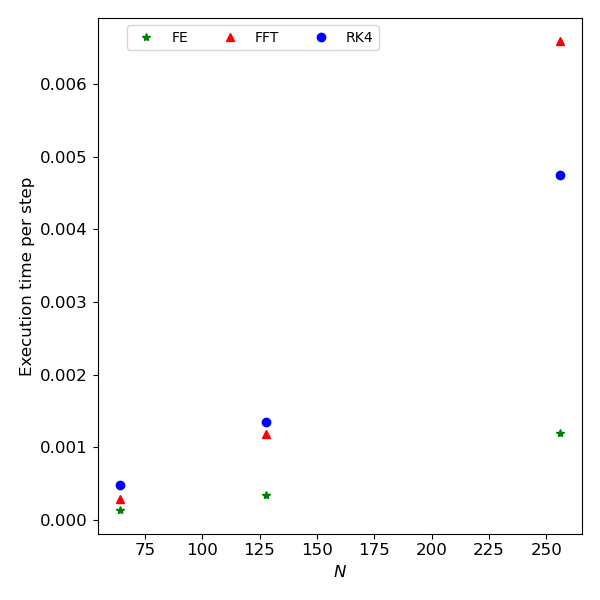
\includegraphics[width=0.5\textwidth]{../figures/AC2D_exec_time.png}
    \caption{Execution times of the various 2D numerical methods}
    \label{fig:2d_exec_time}
\end{figure}

\section{Conclusions}
In this work, I implemented several numerical algorithms for solving the Allen-Cahn equation in 1D and 2D.
The numerical algorithms used were the explicit finite difference forward Euler and fourth-order Runge-Kutta methods, as well as the semi-implicit spectral methods.
These methods were implemented in Python and compared against an analytically tractable toy problem that allowed for error reporting.
It is worth noting that the free energy functionals used in practice are typically always nonlinear to promote phase separation in materials, and that if there are multiple species then solvers would be needed for an Allen-Cahn equation for each species.
Also in the multicomponent case, the free energy functionals would need to account for interfaces between all permutations of species $i$ and species $j$, when $i\neq j$.
Interfacial terms can also be higher order terms in the local expansion of the phase field.
Nonetheless, this work demonstrates applications of principles discussed in lecture to an elementary form of the Allen-Cahn equation.

\newpage
\printbibliography
\end{document}